%%% In this section, you will describe all of the various artifacts that you will generate and maintain during the project life cycle. Describe the purpose of each item below, how the content will be generated, where it will be stored, how often it will be updated, etc. Replace the default text for each section with your own description. Reword this paragraph as appropriate.

\subsection{Major Documentation Deliverables}

\subsubsection{Project Charter}

The project charter will be maintained on a GitHub repository. Updates will be suggested by all members and approved by Luke for pushing to the main branch. The initial version will be delivered by March 19, 2021. At the end of every sprint the team will decide if updates to this document are needed, and who will be in charge of them. Since the document may be updated throughout the whole development cycle of the project, the final version could be delivered during the last sprint in the summer semester, but a "final" version will be delivered at the end of sprint 4 on May 3rd, 2021.

\subsubsection{System Requirements Specification}
Describe how this document will be maintained and updated (how often, under what circumstances, etc.). When will the initial version be delivered? When will the final version be delivered?

The System Requirements Specification (SRS) document will be maintained in an Excel document, shared through Google Drive to allow all members to collaborate on it. This document will be updated at the beginning and end of every sprint unless members decide that there are no updates needed. The initial version will be delivered on March 23rd, 2021, at the beginning of sprint 3. Due to the nature of SCRUM, this document will be constantly evolving, and a final version will not be ready until the team is close to the completion of the project. A somewhat final version will be delivered at the end of sprint 4 on May 3rd, 2021.

\subsubsection{Architectural Design Specification}

The architecural design specification (ADS) will be maintained throughout the development cycle to match the SRS. The initial version will be delivered on April 14, 2021. Any revisions made between then and the end of sprint 4 will result with the delivery of the final version on May 3rd, 2021.This document will be maintained in a GitHub repository where the whole team can see and make updates as needed.

\subsubsection{Detailed Design Specification}

The detailed design specification (DDS) document will be developed and maintainedalong with the ADS due to their similarities, with the goal of delivering the initial and final at the same time as the ADS. This document will be maintained in a GitHub repository where the whole team can see and make updates as needed.
\subsection{Recurring Sprint Items}

\subsubsection{Product Backlog}
How will items be added to the product backlog from the SRS? How will these items be prioritized? Who makes the decision (product owner, group vote, etc.)? What software will be used to maintain and share the product backlog with team members and stakeholders?

The product backlog will be created once the SRS initial version is complete. The team will work during sprint 3 to turn all the requirements from the SRS into products in the product backlog. The products will be listed in a priority order, decided by the team. This priority order may be changed at the end of every sprint if needed. This document will be maintained on a Google Drive file where the whole team can see and make updates as needed.

\subsubsection{Sprint Planning}

The team will meet at the beginning of each sprint to determine the sprint goals, and members will pick products from the product backlog to complete during the sprint. There will be a total of about 7 sprints, 4 in the spring and 3 in the summer. Sprints will be around 2 weeks in lenght, unless the team decides it would be beneficial to change the length.

\subsubsection{Sprint Goal}

The sprint goal will be decided by the team in the sprint planning meeting. This goal will set the theme for what the team will accomplish individually and as a team. Professor Conly will aid in the sprint goal if needed to ensure we are on track with the project goals. Each item will have an expected amount of effort needed, which can be updated at any time.

\subsubsection{Sprint Backlog}

During the sprint planning, the team will decide which items should be completed during the sprint, and put them on a Google Drive document. The items chosen will be decided based on the sprint goal.

\subsubsection{Task Breakdown}

Each team member will pick items from the product backlog at the sprint planning meeting. The rest of the team will give input on the priority and amount of items picked by each member to ensure enough progress is made, as well as not overwhelming people with too many items. The sprint backlog will be maintained and updated on Google Drive.

\subsubsection{Sprint Burn Down Charts}

The sprint burn down charts will be updated at the end of each sprint using the information from the sprint backlog. The graph will be created on Excel to easily access the data from the backlog. No specific person is assigned to this task, rather whoever is done with their tasks and would like to volunteer. We will try to rotate this responsability.

\begin{figure}[h!]
    \centering
    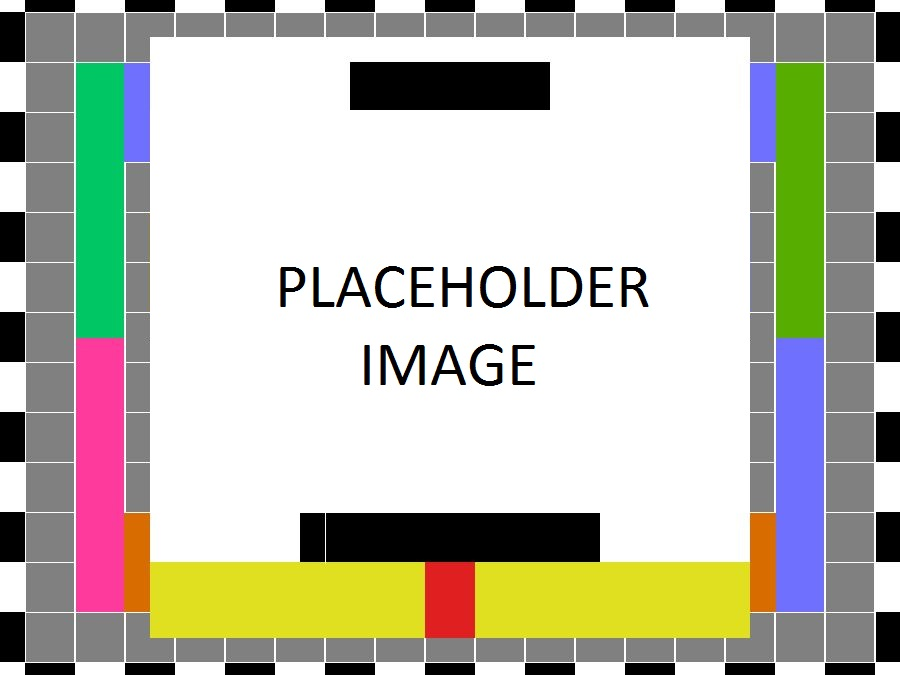
\includegraphics[width=0.5\textwidth]{images/test_image}
    \caption{Example sprint burn down chart}
\end{figure}

\subsubsection{Sprint Retrospective}

At the end of every sprint, the team will meet and take some time to share what they think of the sprint system being implemented. Each team member will share what they think the team should start doing, what the team should stop doing, and what the team should continue to do. The conclusions will be applied on the following sprint.

\subsubsection{Individual Status Reports}

On the weekend landing in the middle of the sprint, each team member will give an update on their current progress for the sprint. The update will contain informatino such as what has been accomplished, what still needs to be accomplished, and any problems encountered that may delay progress. This update will be shared on Discord.

\subsubsection{Engineering Notebooks}

Each member will update their engineering notebook as many times as needed during each sprint, but at least one page per week. Due to the pandemic, each member can choose a family member, roommate, friend, or teammate to sign as a witness if they feel comfortable meeting in person. Pictures of each members progress can be shared on Discord to keep each other accountable.

\subsection{Closeout Materials}

\subsubsection{System Prototype}
What will be included in the final system prototype? How and when will this be demonstrated? Will there be a Prototype Acceptance Test (PAT) with your customer? Will anything be demonstrated off-site? If so, will there be a Field Acceptance Test (FAT)?

\subsubsection{Project Poster}
What will be included on the poster, what will be the final dimensions, and when will it be delivered?

\subsubsection{Web Page}
What will be included on the project web page? Will it be accessible to the public? When will this be delivered? Will it be updated throughout the project, or just provided at closeout (at a minimum, you need to provide a simple web page at the end).

The project web page will contain instructions to brew a patch, as well as information on the current patch.

\subsubsection{Demo Video}
The demo video will be us giving a short explanation of what the brewing process looks like using our project, including the setup, the brewing itself, the monitoring done, and the final product. The video will be short, around 5 minutes or less.

\subsubsection{Source Code}
How will your source code be maintained? What version control system will you adopt? Will source code be provided to the customer, or binaries only? If source code is provided, how will it be turned over to the customer? Will the project be open sourced to the general public? If so, what are the license terms (GNU, GPL, MIT, etc.). Where will the license terms be listed (in each source file, in a single readme file, etc.).

The code will be maintained on GitHub, available to the public. The licence terms will be listed in a readme file on the repository.

\subsubsection{Source Code Documentation}
What documentation standards will be employed? Will you use tools to generate the documentation (Doxygen, Javadocs, etc.). In what format will the final documentation be provided (PDF, browsable HTML, etc.)?

Doxygen will be used to generate documentation and the final documentation will be provided in PDF format.

\subsubsection{Hardware Schematics}
The hardware shematic will be provided once the team has receieved their equipment and have received proper training on how a brewing system should be set up. 



\subsubsection{Installation Scripts}
How will the customer deploy software to new installations? Will you provide installation scripts, install programs, or any other tools to improve the process? Will there be multiple scripts provided (perhaps separate scripts for the graphical front end and back end server software)?

\subsubsection{User Manual}

A digital user manual will be provided.
